\chapter[DESENVOLVIMENTO]{DESENVOLVIMENTO}


%\section{Speech Recognition}
Neste trabalho foi feita a comparação entre duas APIs que realizam a transcrição de áudio para texto, sendo uma delas do Google, conhecida como Cloud Speech-to-Text e a Wit.ai que é utilizada pelo Facebook em bots de chat do messenger. Estas ferramentas processam arquivos de áudio afim de transcrever a fala para texto. Foi utilizado a linguagem Python e a biblioteca Speech Recognition criada por \citeonline{SpeechRecognition} que serve para simplificar a interação do código desenvolvido com a API. Neste capítulo será detalhado como foi implementado o ambiente para análise do desempenho das APIs.

\begin{figure}[h!]
\centering
\caption{Diagrama das APIs selecionadas para análise}
\label{diagramaAPI}
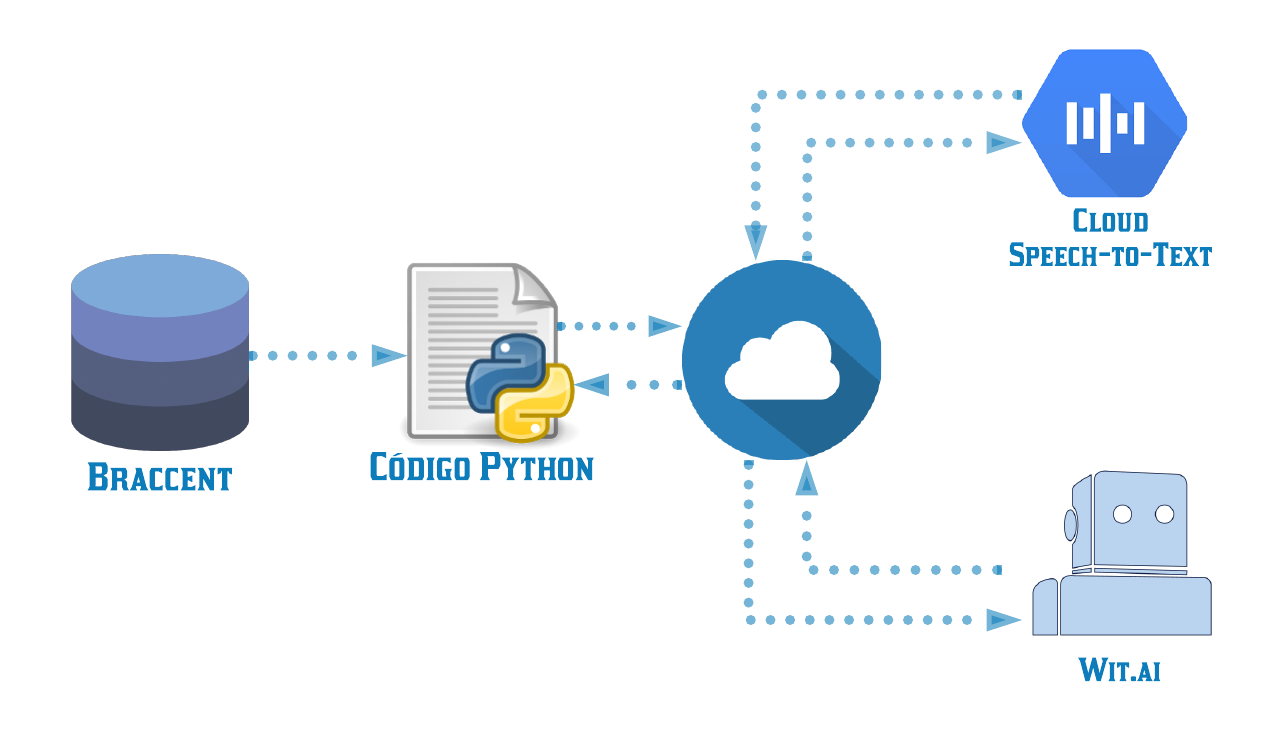
\includegraphics[width=115mm]{images/Diagramas/APIs.png}
\fonte{Elaborado pelo próprio autor (2021).}
\end{figure}

Conforme ilustrado na Figura \ref{diagramaAPI}, o funcionamento do código ocorre de acordo com o seguinte fluxo:

\begin{enumerate}[itemsep=2pt,parsep=2pt]
    \item O código desenvolvido em Python coleta o áudio da base de dados Braccent;
    \item O código Python desenvolvido solicita o processamento do áudio através da nuvem para a respectiva API;
    \item O código fica em modo \emph{stand by} enquanto aguarda a resposta;
    \item A API retorna a resposta;
    \item O código apresenta o texto referente a transcrição do áudio para o usuário;
\end{enumerate}

\section{GOOGLE CLOUD SPEECH API}

A API foi escolhida por ser de uma empresa de  reconhecimento mundial e disponibilizar 300 dólares de crédito com validade de um ano, considerado como suficiente para a conclusão do projeto, além de possuir suporte para o idioma português do Brasil (pt-BR), sendo um requisito obrigatório.

Para começar a utilizá-la é necessário fazer o download da biblioteca através do comando 'pip install google-api-python-client' no prompt de comando, e então criar uma conta no \emph{Google Cloud Platform}, através do link \footnote{https://cloud.google.com/speech-to-text}, clicando no botão 'Comece a usar gratuitamente' no canto superior direito como é possível observar na Figura \ref{Cloudexplicação}, que vai redirecionar para uma tela em que deve acessar uma conta do Google e então preencher um formulário de cadastro composto por duas etapas. 


\begin{figure}[h!]
\centering
\caption{Tela explicativa da Cloud Speech-to-Text}
\label{Cloudexplicação}
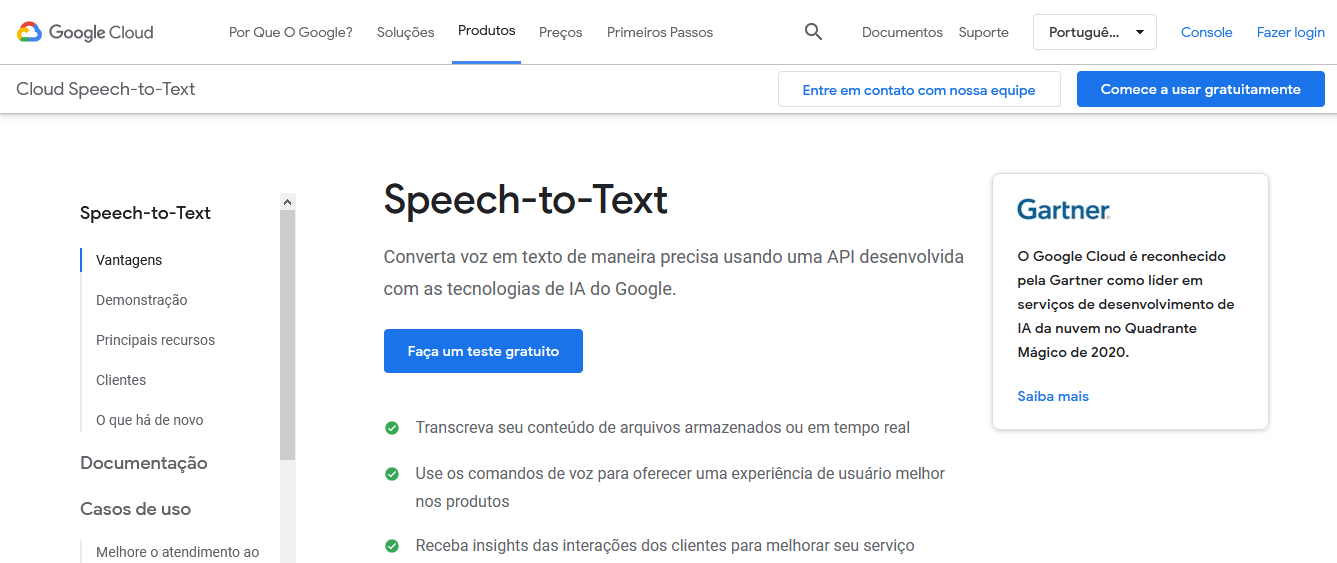
\includegraphics[width=140mm]{images/ConfigurarGoogle/Google_TelaInicial.PNG}
\fonte{Elaborado pelo próprio autor (2021).}
\end{figure}


Na etapa 1 deve ser informado (Figura \ref{CloudCadastro1}) o país de onde vai acessar e ler e concordar com os termos ``Custom Search API Termos de Serviço'' e ``Termos de Serviço do período de teste gratuito do Google Cloud Platform''. Feito isso e pressionando o botão continuar, são solicitados seus dados de endereço (Figura \ref{CloudCadastro2a} e forma de pagamento Figura \ref{CloudCadastro2b}).

\begin{figure}[h!]
\centering
\caption{Tela de Cadastro da Cloud Speech-to-Text, etapa 1}
\label{CloudCadastro1}
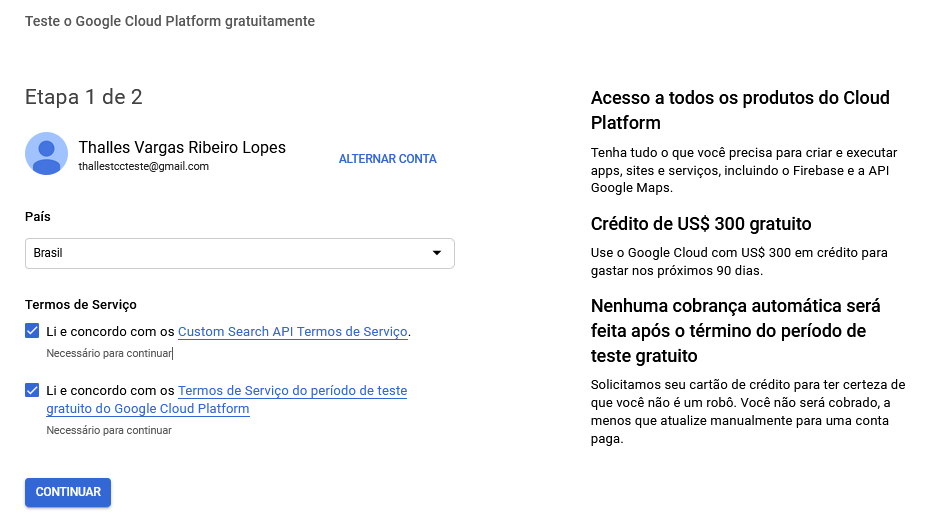
\includegraphics[width=140mm]{images/ConfigurarGoogle/cadastroetapa01.PNG}
\fonte{tela do Google Cloud (2021).}
\end{figure}

\begin{figure}[h!]
\centering
\caption{Tela de Cadastro da Cloud Speech-to-Text, etapa 2A}
\label{CloudCadastro2a}
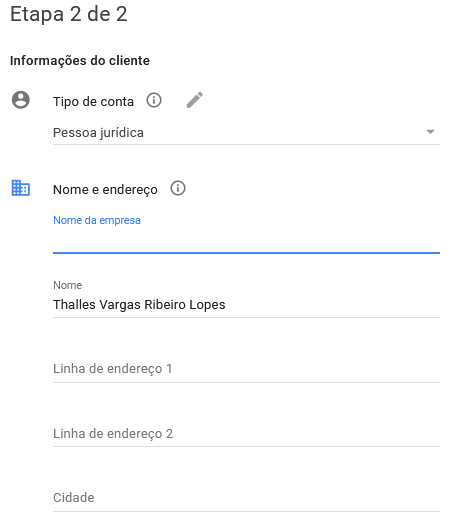
\includegraphics[width=80mm]{images/ConfigurarGoogle/cadastroetapa02a.PNG}
\fonte{tela do Google Cloud (2021).}
\end{figure}

\begin{figure}[h!]
\centering
\caption{Tela de Cadastro da Cloud Speech-to-Text, etapa 2B}
\label{CloudCadastro2b}
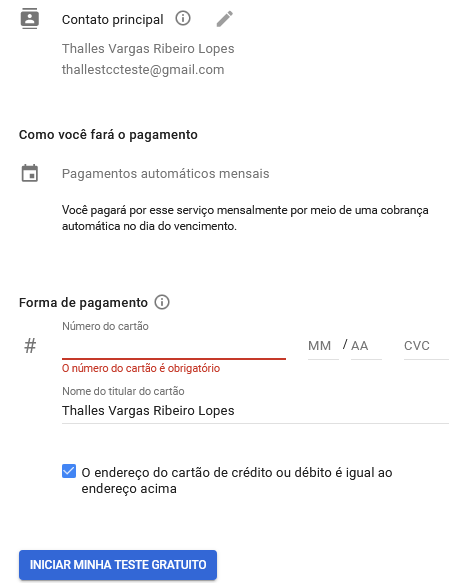
\includegraphics[width=80mm]{images/ConfigurarGoogle/cadastroetapa02b.PNG}
\fonte{tela do Google Cloud (2021).}
\end{figure}
\FloatBarrier


Com a conta criada e com acesso a plataforma do Google, basta realizar a busca no campo que se encontra na parte de cima da tela (Figura \ref{plataformaGoogle}) digitando 'Speech-to-Text e ativar a ferramenta em seu perfil pressionando o comando 'Ativar' (Figura \ref{AtivarAPI}), feito isso, terá acesso ao ambiente de configuração da sua API (Figura \ref{telainicialAPI}) onde deve acessar o menu 'Credenciais' e preencher os campos necessários (Figuras \ref{criarCredencial} e \ref{criarCredencial2}) para receber a credencial que vai ser utilizada na chamada da API (Figura \ref{chaveCriada}).

\begin{figure}[h!]
\centering
\caption{Tela Inicial da Plataforma Google}
\label{plataformaGoogle}
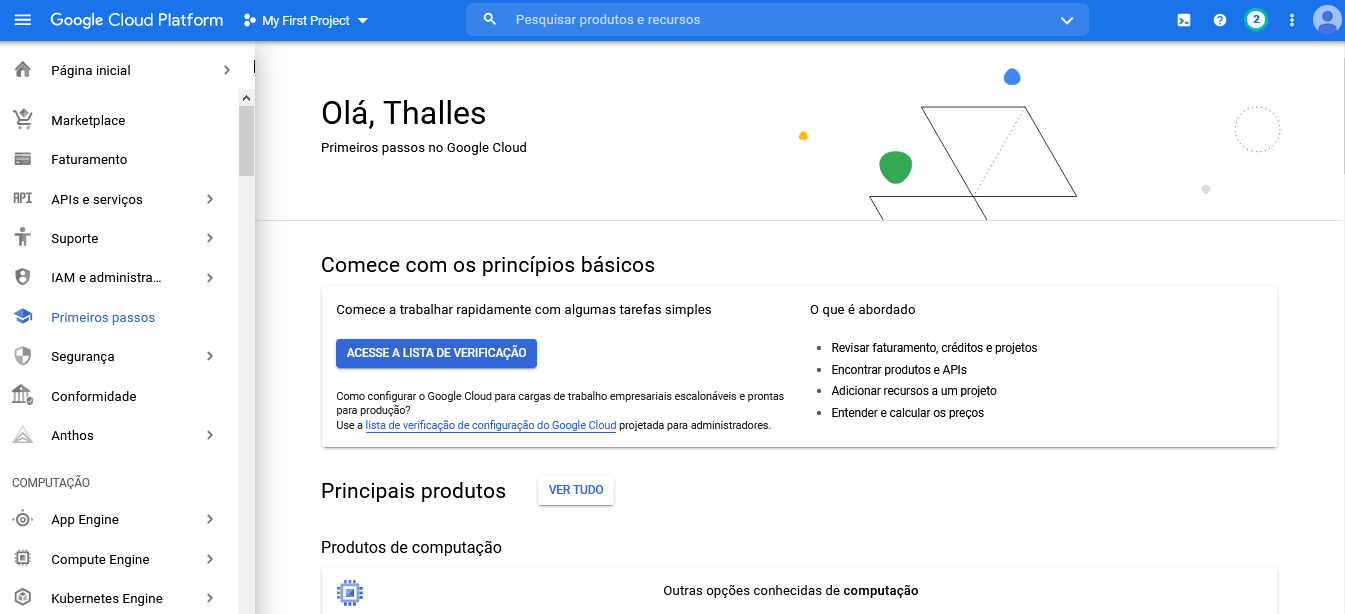
\includegraphics[width=150mm]{images/ConfigurarGoogle/telainicial.PNG}
\fonte{tela do Google Cloud (2021).}
\end{figure}

\begin{figure}[h!]
\centering
\caption{Tela para Ativar a API Speech-To-Text na conta}
\label{AtivarAPI}
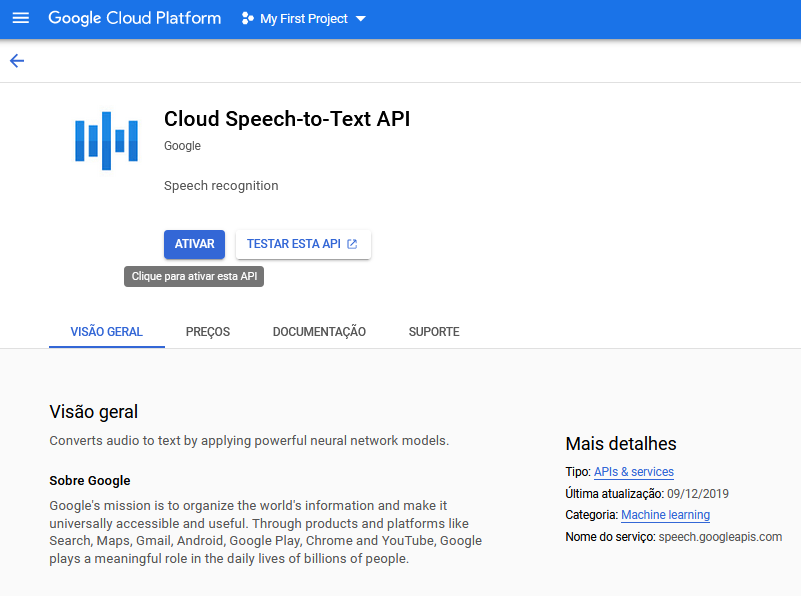
\includegraphics[width=150mm]{images/ConfigurarGoogle/AtivarAPI.PNG}
\fonte{tela do Google Cloud (2021).}
\end{figure}

\begin{figure}[h!]
\centering
\caption{Tela inicial da API Speech-To-Text}
\label{telainicialAPI}
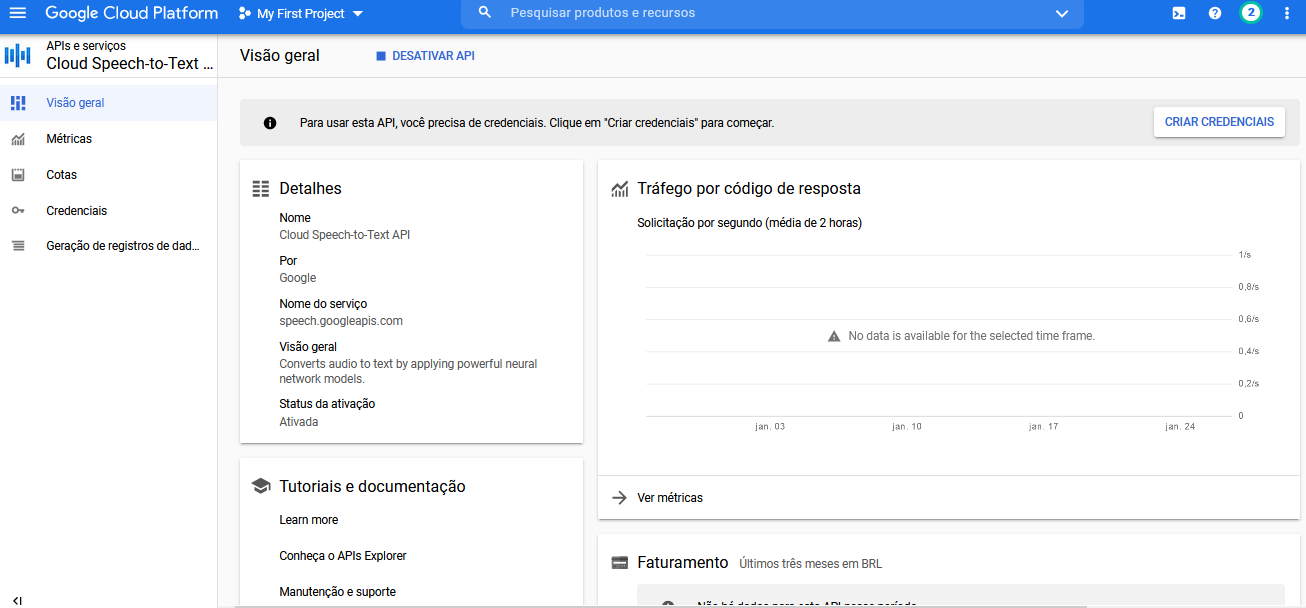
\includegraphics[width=150mm]{images/ConfigurarGoogle/telainicialSpeechToText.PNG}
\fonte{tela do Google Cloud (2021).}
\end{figure}

\begin{figure}[h!]
\centering
\caption{Tela de cadastro de Credencial da API Speech-To-Text, etapa 01}
\label{criarCredencial}
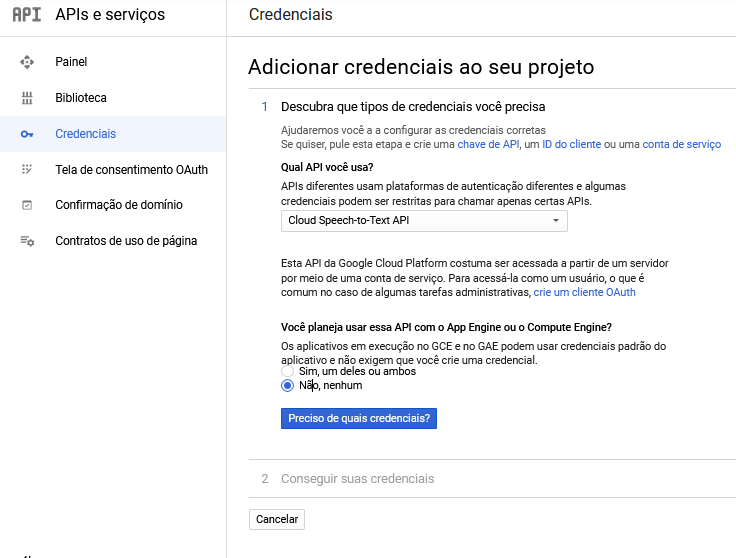
\includegraphics[width=150mm]{images/ConfigurarGoogle/criarCredencialEtapa1.PNG}
\fonte{tela do Google Cloud (2021).}
\end{figure}

\begin{figure}[h!]
\centering
\caption{Tela de cadastro de Credencial da API Speech-To-Text, etapa 02}
\label{criarCredencial2}
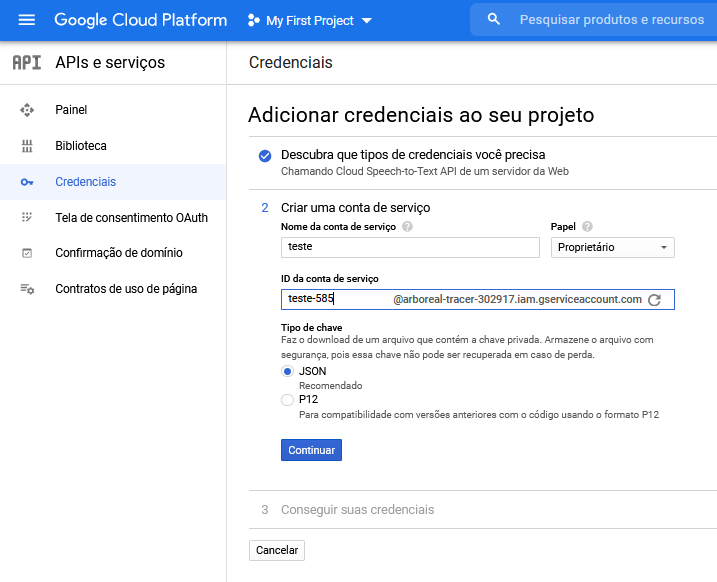
\includegraphics[width=150mm]{images/ConfigurarGoogle/criarCredencialEtapa2.PNG}
\fonte{tela do Google Cloud (2021).}
\end{figure}

\begin{figure}[h!]
\centering
\caption{Tela de sucesso da criação de credencial}
\label{chaveCriada}
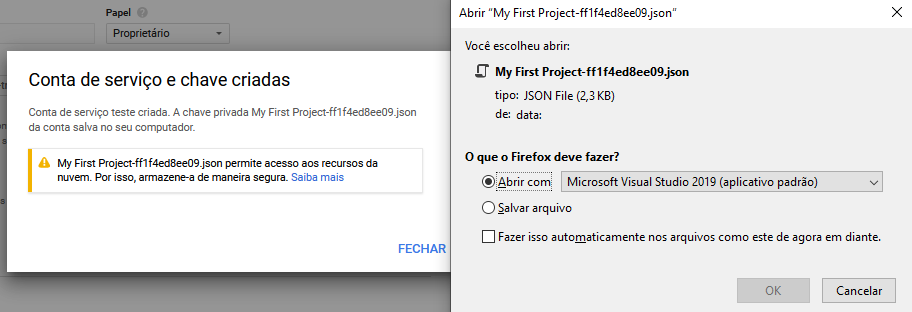
\includegraphics[width=150mm]{images/ConfigurarGoogle/chaveCriada.PNG}
\fonte{tela do Google Cloud (2021).}
\end{figure}

\FloatBarrier

O código descrito no \autoref{googleCloudAPI} demonstra a chamada da API para os testes do projeto. Iniciando importando a biblioteca Speech Recognition que vai realizar o intermédio entre a API e o programa. Na linha 5 é passado o caminho para a pasta que a base dados BRACCENT se encontra. Na linha 6 deve ser atribuído à variável ``GOOGLE\_CLOUD\_SPEECH\_CREDENCIALS'' a credencial gerada na plataforma do Google. Na linha 8 é iniciado um \textit{loop} que deve verificar todos os arquivos que se encontram no diretório passado como parâmetro e então enviar todos que forem arquivos '.wav' para a API do Google realizar a transcrição. Na requisição na linha 17 e 18, passam-se como parâmetros o áudio, a língua que está sendo transcrita e as credenciais, e o processo fica aguardando a resposta da API. Se a chave e o áudio fornecidos forem válidos, é retornado a resposta em formato de \textit{string}. 

\begin{quadro}[h!]
\centering
\caption{Código para realizar a chamada da API \emph{Google Cloud API}}
\label{googleCloudAPI}
\lstdefinestyle{nonumbers}
{numbers=none}
\begin{lstlisting}[language=Python]
import speech_recognition as sr
from os import path
import os

directory = r'C:\TCC\BRAccent001\Stereo\Baiano\Masculino'
GOOGLE_CLOUD_SPEECH_CREDENTIALS = ''KEY''

for filename in os.listdir(directory):
    if filename.endswith('.wav'):
        AUDIO_FILE = path.join(directory, filename)

        r = sr.Recognizer()
        with sr.AudioFile(AUDIO_FILE) as source:
            audio = r.record(source)
            
        try:
            print(r.recognize_google_cloud(audio, language='pt-BR', credentials_json=GOOGLE_CLOUD_SPEECH_CREDENTIALS))
        except sr.UnknownValueError:
            print(''Google Cloud Speech could not understand audio'')
        except sr.RequestError as e:
            print(''Could not request results from Google Cloud Speech service; {0}''.format(e))
\end{lstlisting}
\fonte{Elaborado pelo autor (2021).}
\end{quadro}

Caso finalize a resposta sem nenhum erro, é retornado o texto ou a \textit{string} do áudio. Existem duas exceções definidas para possíveis problemas, o primeiro para o caso da API do Google não conseguir identificar quais palavras estão sendo pronunciadas (linha 18) e o segundo para o erro de conexão com a API (Linha 20). 

\section{WIT.AI}

A {Wit.ai} foi selecionada pela sua  facilidade de uso, ser completamente gratuita e possuir suporte para o idioma português do Brasil (pt-BR). A empresa  somente solicita que seja informada no caso em que há chamadas com muita frequência, por exemplo, uma  chamada por segundo. Neste trabalho não foi necessário o uso intenso da API e portanto não houve essa notificação.

Para começar a utilizá-lo deve acessar o site\footnote{https://wit.ai} e realizar o cadastro através de uma conta do Facebook ou Github, conforme é possível ver na parte inferior direita da Figura \ref{witInicio}. Após ter acessado a conta é apresentada a listagem de suas aplicações (Apps) criadas (Figura \ref{witListagemApps}), no caso de ser a primeira deve ser acessado o botão '\textbf{+ New App}' que vai abrir a tela de cadastro de App (Figura \ref{witCreateApp}) onde é necessário informar o nome da App, a linguagem que vai ser utilizada na transcrição e a privacidade da App. 

\begin{figure}[h!]
\centering
\caption{Tela inicial do site Wit.ai}
\label{witInicio}
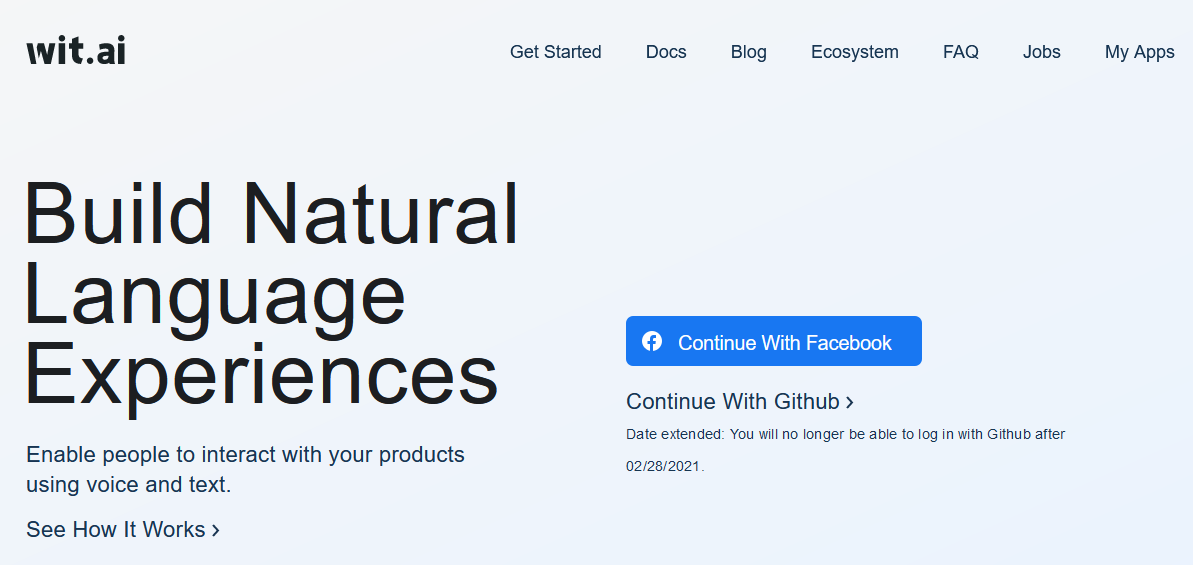
\includegraphics[width=150mm]{images/ConfigurarWit/witTelaInicial.PNG}
\fonte{tela do Wit.ai (2021).}
\end{figure}

\begin{figure}[h!]
\centering
\caption{Tela de listagem das Apps da conta Wit}
\label{witListagemApps}
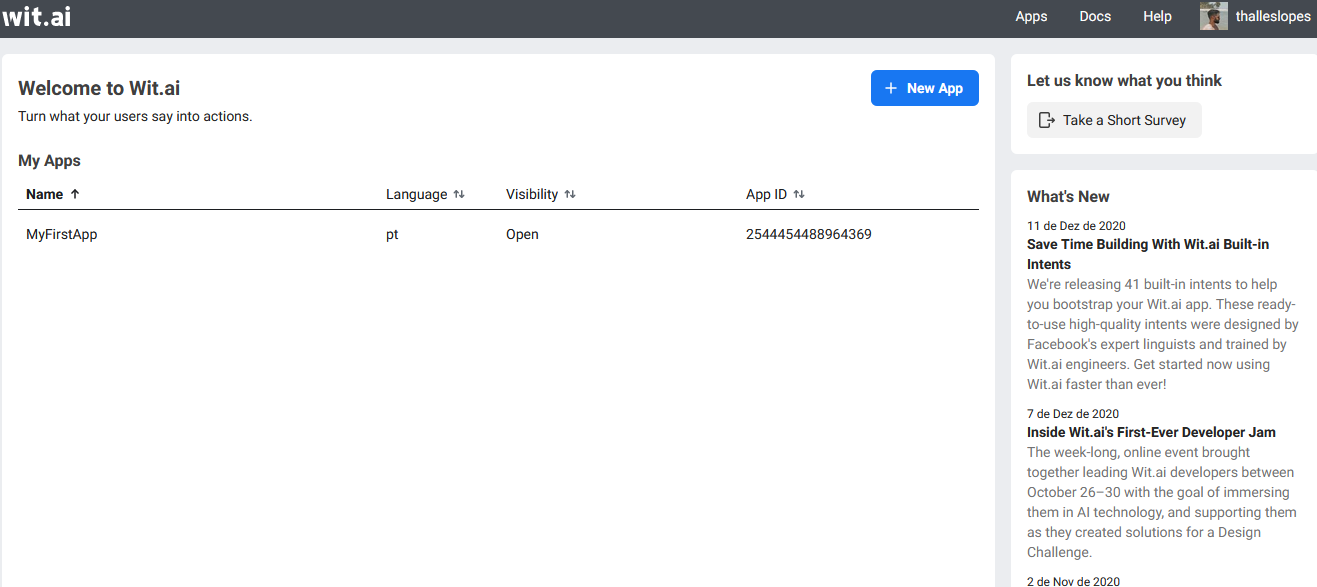
\includegraphics[width=150mm]{images/ConfigurarWit/witListagemApp.PNG}
\fonte{tela do Wit.ai (2021).}
\end{figure}

\begin{figure}[h!]
\centering
\caption{Tela de cadastro de App da Wit}
\label{witCreateApp}
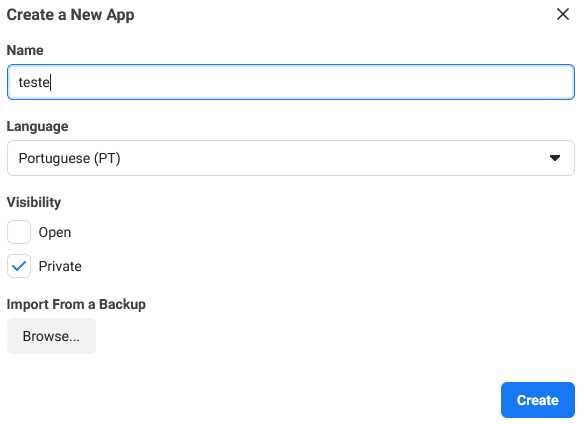
\includegraphics[width=100mm]{images/ConfigurarWit/witCreateApp.PNG}
\fonte{tela do Wit.ai (2021).}
\end{figure}

\FloatBarrier
Clicando no botão \textbf{Create} para confirmar a criação, o usuário é  redirecionado  para a tela inicial da App (Figura \ref{witAppInicio}) que apresenta o histórico de transcrições realizadas, caso tenha acabado de criar a App, nenhum dado vai ser apresentado. Acessando o menu na lateral esquerda, '\textbf{Settings}' dentro de '\textbf{Management}', são apresentadas as configurações da App (Figura \ref{witAppSettings}), onde permite configurar informações referentes a App, como por exemplo o '\textbf{Server Acess Token}' que é necessário para realizar a chamada da API.



\begin{figure}[h!]
\centering
\caption{Tela Inicial da App da Wit.ai}
\label{witAppInicio}
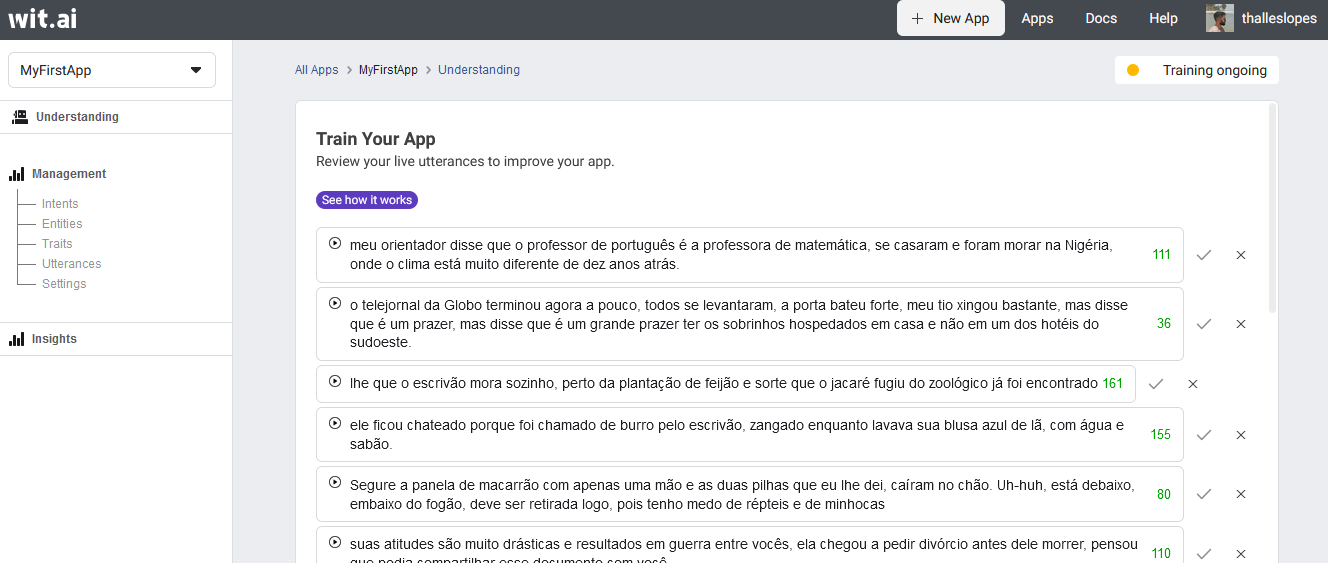
\includegraphics[width=160mm]{images/ConfigurarWit/witHistoricoTranscricao.PNG}
\fonte{tela do Wit.ai (2021).}
\end{figure}

\begin{figure}[h!]
\centering
\caption{Tela de configuração da App da Wit.ai}
\label{witAppSettings}
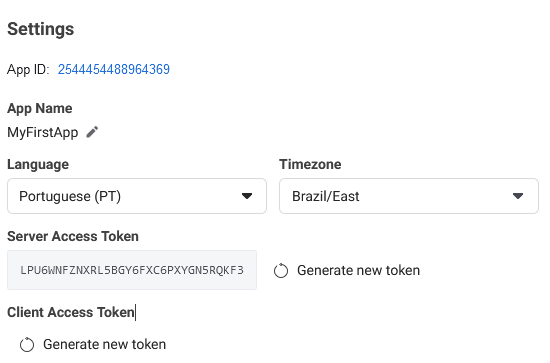
\includegraphics[width=110mm]{images/ConfigurarWit/witSettings.PNG}
\fonte{tela do Wit.ai (2021).}
\end{figure}

\FloatBarrier

Com o \textit{token} gerado já é possível utilizar a biblioteca Speech Recognition para a transcrição com a Wit. No Quadro \autoref{witAPI} apresenta o código de chamada da API, que funciona de maneira similar à do Google Cloud.


\begin{quadro}[h]
\centering
\caption{Código para realizar a chamada da API \emph{Wit.ai}}
\label{witAPI}
\lstdefinestyle{nonumbers}
{numbers=none}
\begin{lstlisting}[language=Python]
import speech_recognition as sr
from os import path
import os
directory = r'C:\TCC\BRAccent001\Mono\Baiano\Feminino'

WIT_AI_KEY = "Wit.ai_key" 

for filename in os.listdir(directory):
    if filename.endswith(".wav"):
        AUDIO_FILE = path.join(directory, filename)

        r = sr.Recognizer()
        with sr.AudioFile(AUDIO_FILE) as source:
            audio = r.record(source) 

        try:	
            print(r.recognize_wit(audio, key=WIT_AI_KEY))
        except sr.UnknownValueError:
            print("Wit.ai could not understand audio")
        except sr.RequestError as e:
            print("Could not request results from Wit.ai service; {0}".format(e))
            
\end{lstlisting}
\fonte{Elaborado pelo autor (2021).}
\end{quadro}

O código inicia importando a biblioteca Speech Recognition que vai realizar o intermédio entre a API e o programa. Na linha 4 é passado o caminho para a pasta que a base dados BRACCENT se encontra. Na linha 6 deve ser atribuído à variável ''WIT\_AI\_KEY'' o \textit{token} gerado na plataforma da Wit. Na linha 8 é iniciado um \textit{loop} que deve verificar todos os arquivos que se encontram no diretório passado como parâmetro e então enviar todos que forem arquivos '.wav' para a API da Wit realizar a transcrição. 

 
Ao realizar a requisição na linha 18, passando como parâmetros o áudio e a chave, o processo fica parado aguardando a resposta da API (o parâmetro de língua é mantido nas configurações da App). Se a chave e o áudio fornecidos forem válidos, é retornada a resposta em formato de \textit{string}.

\section{TRATAMENTO DE PONTUAÇÃO}

Posteriormente ao inicio do trabalho, foi feito o processamento das transcrições para remover as pontuações, afim de produzir duas planilhas distintas para serem analisadas, conforme a necessidade de realizar uma comparação mais equivalente, uma vez que o Google Cloud não realiza a utilização de pontuação.

Como é possível observar no \autoref{removerPontuacao}, nas linhas 1 e 2 são importadas as bibliotecas necessárias para manipular as planilhas. Na linha 4 é selecionado a planilha que possui os dados para serem tratados e na linha 5 a aba da planilha. Na linha 6 são definidos todas as pontuações que devem ser removidas do texto. Na linha 8 é realizado um loop para percorrer todas as células que possuem o texto verificando se algum dos caracteres é trata de uma pontuação, se for o caso ela deve ser removida (substituída por uma String vazia). Após percorrer todos os caracteres do texto o código deve ajustar todas as letras para minúscula, através do comando feito na linha 14.

\begin{quadro}[h]
\centering
\caption{Código para remover a pontuação \emph{Wit.ai}}
\label{removerPontuacao}
\lstdefinestyle{nonumbers}
{numbers=none}
\begin{lstlisting}[language=Python]
import openpyxl
from openpyxl import load_workbook

wb = load_workbook(filename = ''2 Google Cloud - BRACCENT.xlsx'')
ws = wb['Sulista']
pontuacao = '''!()-[]{};:'"\,<>./?@#$%^&*_~'''

for row in ws.iter_rows(min_row=2, max_col=4, max_row=1000, values_only=True):
    frase = row[2]
    for ele in frase:  
        if ele in pontuacao:  
            frase = frase.replace(ele, '')  
    
    frase = frase.lower()
    print(frase)
\end{lstlisting}
\fonte{Elaborado pelo autor (2021).}
\end{quadro}



\section{COLETA DAS MÉTRICAS DE COMPARAÇÃO}

Para a coleta das métricas de comparação de texto, existem dois resultados diferenciados: considerando a pontuação e sem considerar a pontuação. A pontuação das frases são as vírgulas, pontos finais, aspas e parágrafos (letra maiúscula). O resultado da ferramenta Google Cloud não utiliza quaisquer tipos de pontuação, diferente da ferramenta Wit.ai em que sua transcrição contém vírgulas, pontos finais e letras maiúsculas de início de parágrafo. O Wit.ai só não avalia as aspas. 

%\todo[inline]{como referenciar links?}
Para calcular a similaridade das transcrições feitas pelas API's com as respectivas frases originais, foi utilizada a biblioteca 'python-string-similarity'\footnote{\url{ https://github.com/luozhouyang/python-string-similarity\#python-string-similarity}} que fornece diversas funções para comparar duas \textit{strings}. Para começar a utilizar a biblioteca é necessário fazer o \textit{download}  através do \textbf{cmd} com o comando \textbf{pip install -U strsimpy}. Terminando a instalação, o Python já está configurado para a utilização das funções da biblioteca.


\begin{quadro}[h]
\centering
\caption{Código para calcular a similaridade \emph{Wit.ai}}
\label{métricaLev}
\lstdefinestyle{nonumbers}
{numbers=none}
\begin{lstlisting}[language=Python]
import openpyxl
from openpyxl import load_workbook
from strsimpy.jaro_winkler import Levenshtein

wb = load_workbook(filename = ''Google Cloud - BRACCENT.xlsx'')
ws = wb[''Sulista'']

levenshtein = Levenshtein()
for row in ws.iter_rows(min_row=1, max_col=3, max_row=1000, values_only=True):
    print(levenshtein.distance(row[1], row[2]))
\end{lstlisting}
\fonte{Elaborado pelo autor (2021).}
\end{quadro}


O código utilizado para comparar o resultado das API's é apresentado no \autoref{métricaLev}. Nas Linhas 1, 2 apenas são realizadas importações necessárias para leitura do arquivo XLS e na Linha 3 é feita a importação da métrica Levenshtein da biblioteca \textbf{strsimpy}. Na Linha 5 é selecionado o arquivo para ser lido e na Linha 6 a aba da planilha. A Linha 10 é  um \textit{loop} que vai rodar da primeira linha (\textbf{min\_row=1}) e terceira coluna (\textbf{max\_col=3}) até a linha mil (\textbf{max\_row=1000}) imprimindo o resultado do cálculo de similaridade entre a coluna referente a frase original (\textbf{row[1]}) e a transcrição da API (\textbf{row[2]}).

Há variações deste código na Linha 5, em que o nome do arquivo é alterado para o resultado do Google Cloud sem pontuação, e para o Wit.ai, com e sem pontuação. As abas também são alteradas na Linha 6. E para se fazer o cálculo do Levenshtein normalizado, a Linha 3 e Linha 8 são alteradas como mostrado no Quadro \ref{métricaNormalizedLev}.


\begin{quadro}[h]
\centering
\caption{Código para calcular a similaridade \emph{Wit.ai}}
\label{métricaNormalizedLev}
\lstdefinestyle{nonumbers}
{numbers=none}
\begin{lstlisting}[language=Python]
import openpyxl
from openpyxl import load_workbook
from strsimpy.normalized_levenshtein import NormalizedLevenshtein

wb = load_workbook(filename = ''2 Wit - BRACCENT.xlsx'')
ws = wb[''Sulista'']

normalized_levenshtein = NormalizedLevenshtein()
for row in ws.iter_rows(min_row=2, max_col=4, max_row=1000, values_only=True):
    print(normalized_levenshtein.similarity(row[1], row[2]))
\end{lstlisting}
\fonte{Elaborado pelo autor (2021).}
\end{quadro}



\vspace*{\fill}

{~~~~~~~~~}


{~~~~~~~~~}


